\documentclass[10 pt,usenames,dvipsnames, oneside]{article}
\usepackage{../../../modelo-ensino-medio}



\begin{document}

\begin{center}
  \begin{minipage}[l]{3cm}

\includegraphics[width=2cm]{logo}    
\end{minipage}\hfill
\begin{minipage}[r]{.8\textwidth}
 {\Large \scshape Atividade: Fazendo Mais Bolos}  
\end{minipage}
\end{center}
\vspace{.2cm}

\ifdefined\prof
%Habilidades da BNCC
% \begin{objetivos}
% \item 
% \end{objetivos}

%Caixa do Para o Professor
\begin{goals}
%Objetivos específicos
\begin{enumerate}
\item Resolver um sistema de equações lineares de duas incógnitas.
\item Abordagem geométrica ao problema de solução de sistema de equações lineares de duas incógnitas. 
\end{enumerate}

\tcblower

%Orientações e sugestões
Nessa atividade o aluno deverá encontrar a solução para um sistema de equações lineares de duas incógnitas. Como nenhum método de resolução foi apresentado ainda, recomenda-se que, ao se fazer os gráficos (no item c), os alunos testem valores que pareçam estar próximos ao ponto de interseção das retas.
\end{goals}

\bigskip
\begin{center}
{\large \scshape Atividade}
\end{center}
\fi

Vamos voltar à fábrica de bolos da Tia Tatá? Sabemos que os bolos que mais vendem são os de fubá e o de chocolate e que custam $15$ reais e $18$ reais cada um, respectivamente.

\begin{figure}[H]
\centering

\noindent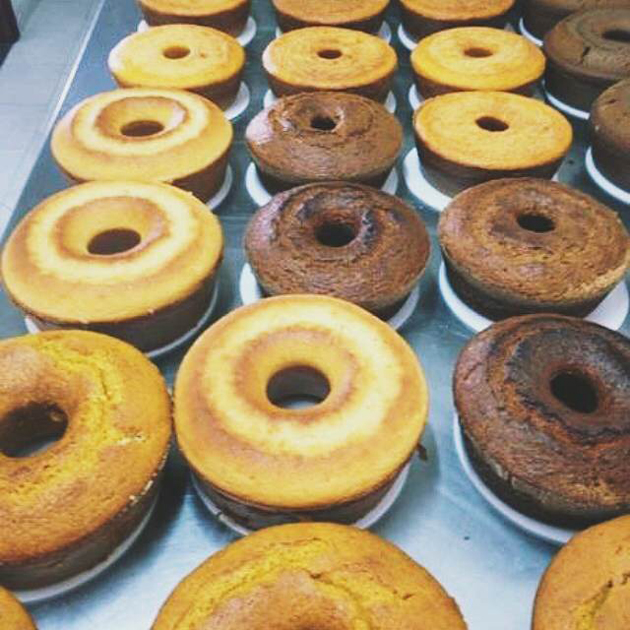
\includegraphics[width=250bp]{bolos.jpg}
\end{figure}

\begin{enumerate}
\item{}
Em determinado dia, a fábrica precisa faturar exatamente R\$ $510{,}00$ com a venda desses dois tipos de bolo. Escreva uma equação que relacione as possíveis quantidades de cada bolo que ela precisa vender;

\item{}
Na receita do bolo de chocolate usam-se $4$ ovos, enquanto na de fubá, usam-se $3$. Escreva uma equação que relacione a quantidade de bolos de chocolate e a quantidade de bolos de fubá e com um total de $100$ ovos;

\item{}
Num mesmo plano cartesiano, faça um esboço das representações gráficas dos conjuntos soluções das equações encontradas nos itens \titem{a)} e \titem{b)};

\item{}
Imagine que o dia em que é necessário se obter o faturamento de R\$ $510{,}00$ é o mesmo em que a fábrica dispõe dos 100 ovos. Assumindo que todos os bolos sejam vendidos, quantos bolos de cada sabor deverão ser produzidos?
\end{enumerate}

\ifdefined\prof
\begin{solucao}

\begin{enumerate}
\item Sendo $x$ a quantidade de bolos de fubá e $y$ a de chocolate
\item $15x+18y =510$.
\item $4x+3y=100$
\item Incentive os alunos a que explorem tanto por construção usando lápis e papel quanto também que utilizem ambientes digitais, como o GeoGebra, por exemplo.
\item $10$ de fubá e $20$ de chocolate.
\end{enumerate}

\end{solucao}
\fi

\end{document}